% %%%%%%%%%%%%%%%%%%%%%%%%%% Figure Map_location_Oslofjord %%%%%%%%%%%%%%%%%%%%%%%%%%%%
\begin{figure}[h]
 \setlength{\unitlength}{1.0cm}
 \begin{center}
  \begin{pspicture}(0,0)(15,9)
% Include graphs
   \rput[bl](-0.2,0.0){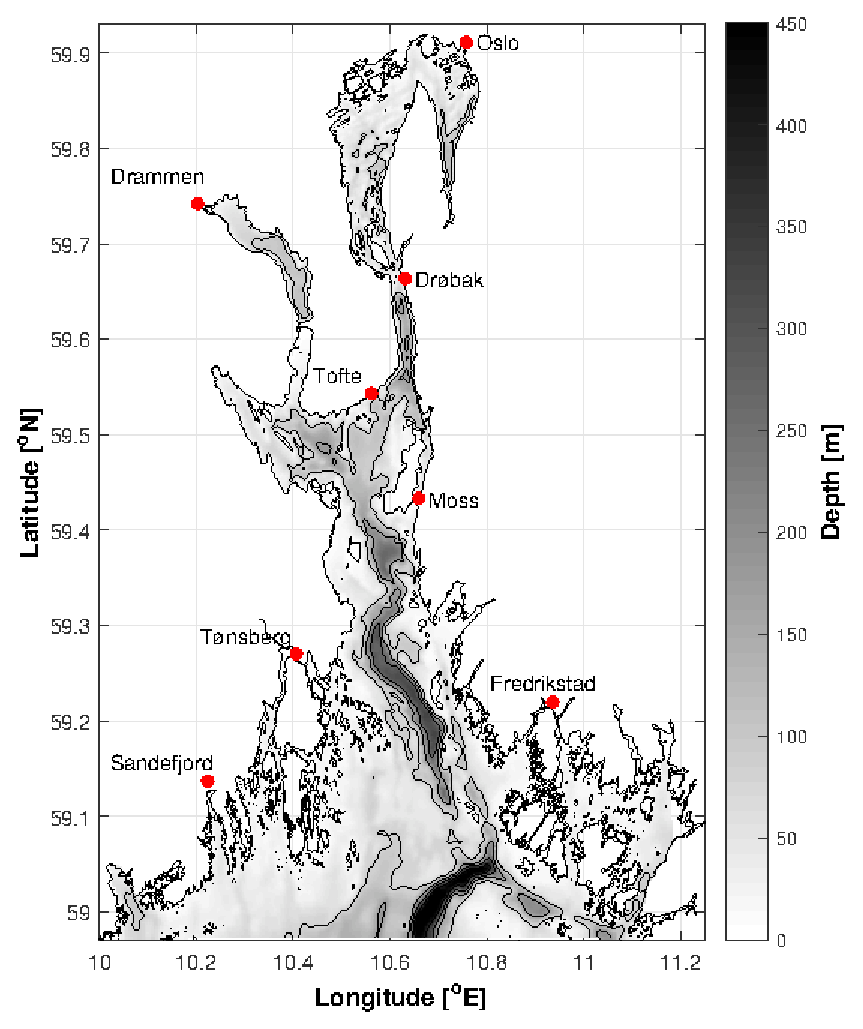
\includegraphics[height=9cm]{dyp}}
%   \rput[bl]( 0.5,0.0){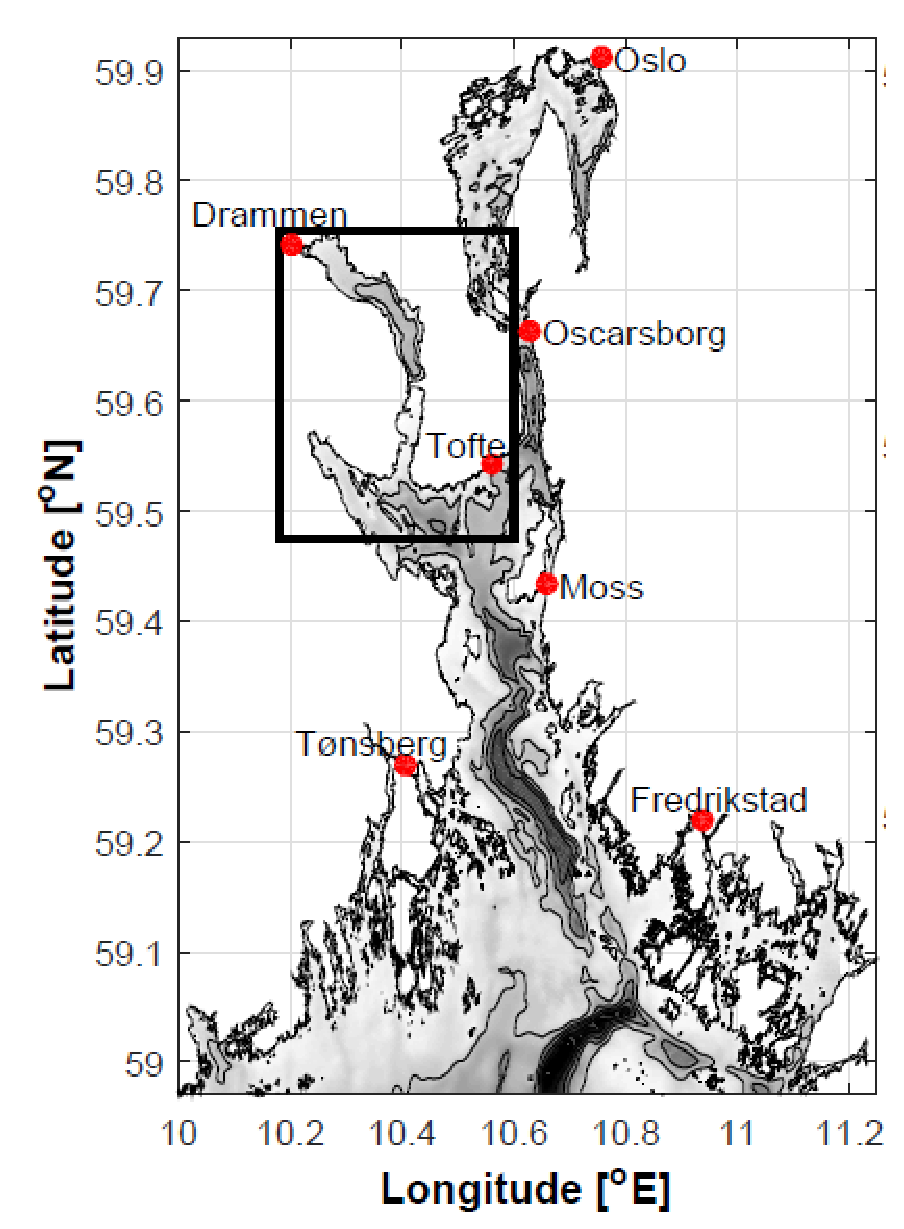
\includegraphics[height=9cm]{Map_Oslofjord_with_topography}}
%   \rput[bl]( 7.5,0.0){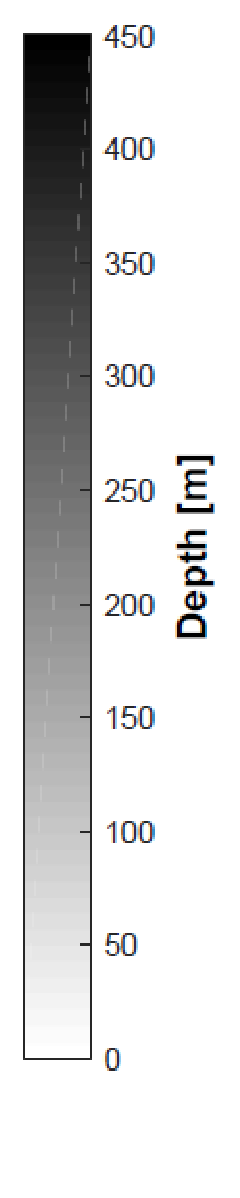
\includegraphics[height=9cm]{Fig01_2}}
   \rput[br](15.0,1.0){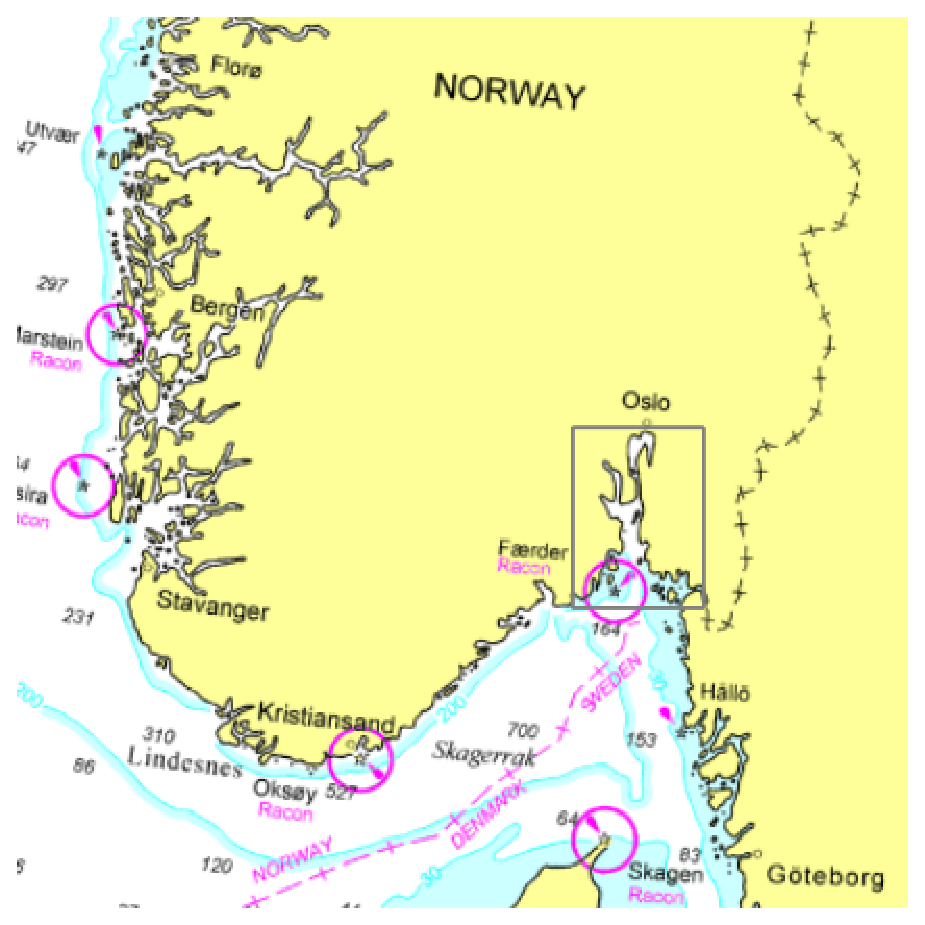
\includegraphics[height=7.3cm]{Map_location_Oslofjord_2}}
   \psline[linewidth=0.5mm,linecolor=blue]{->}(1.4,6.3)(3.3,6.3)
%   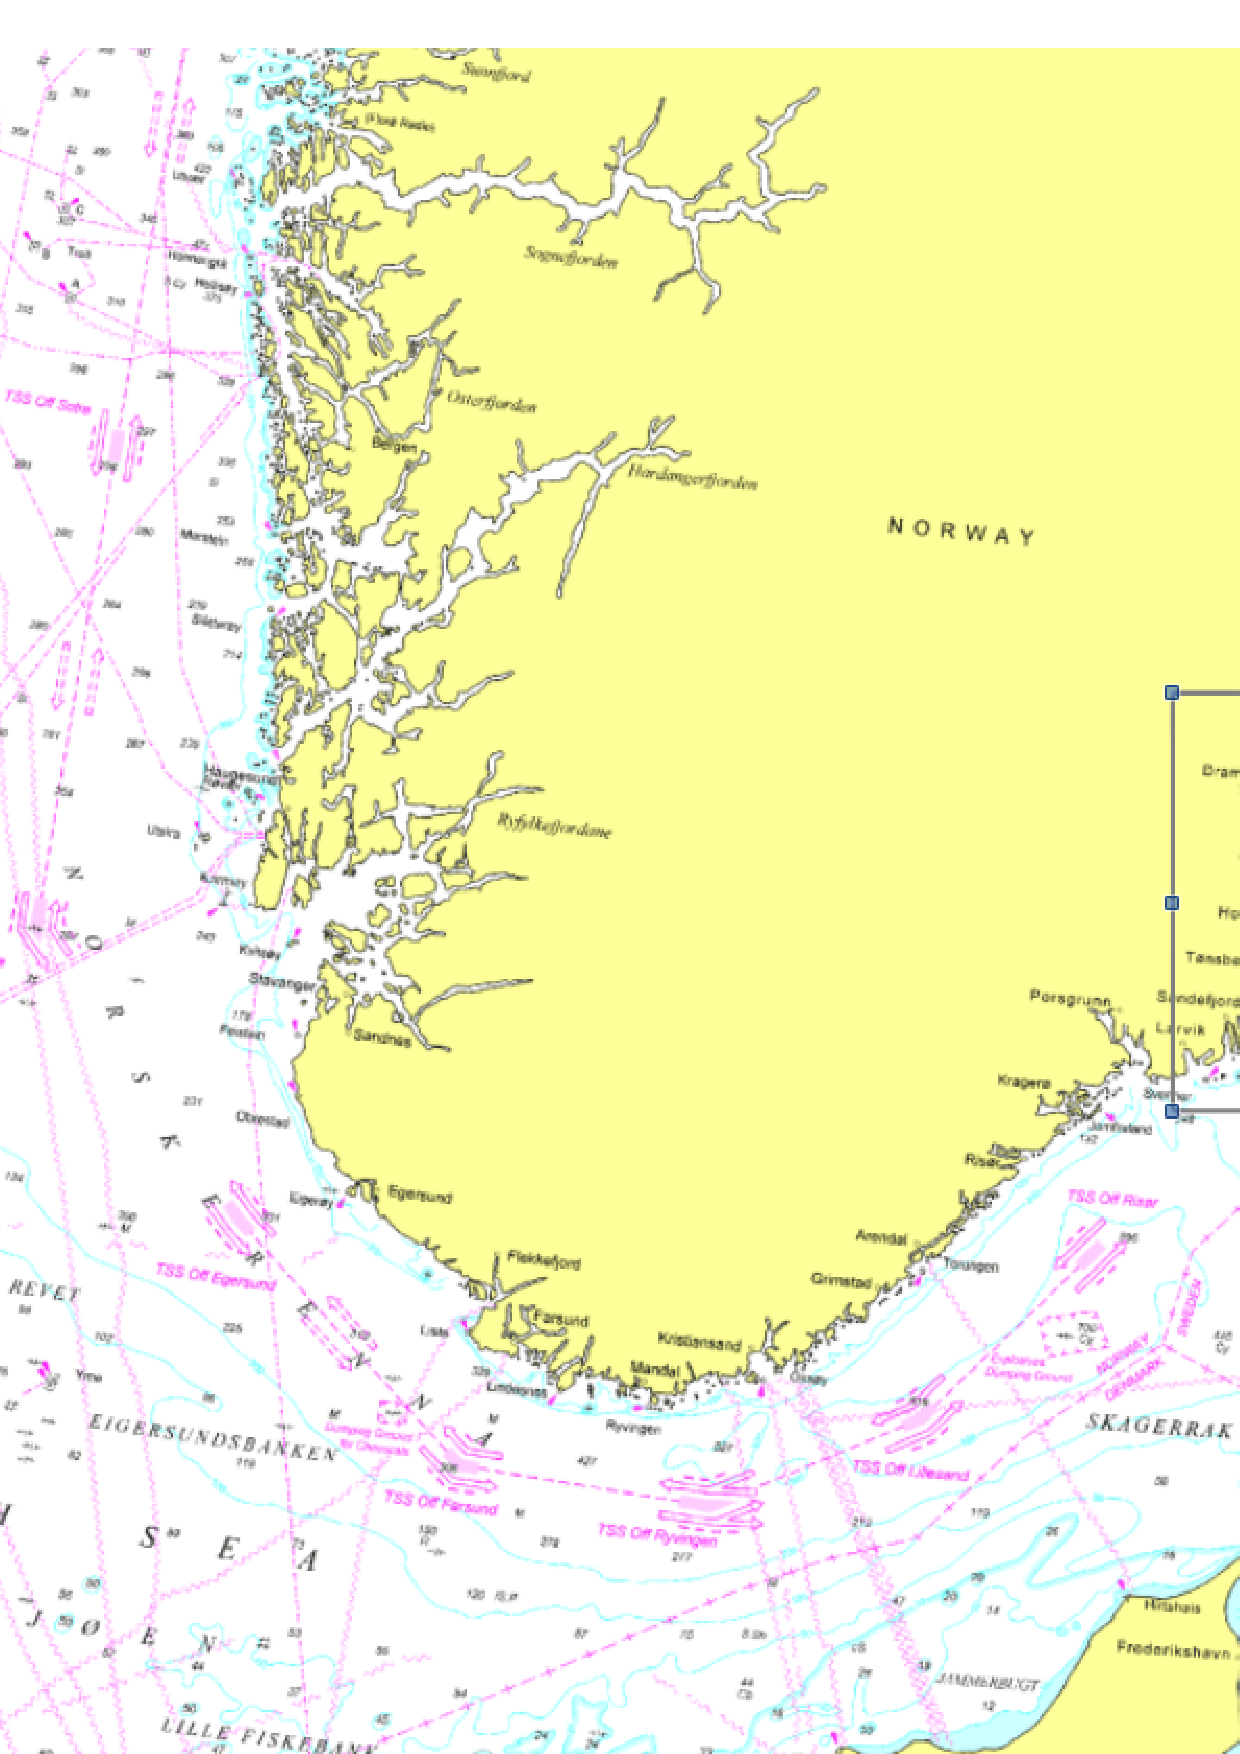
\includegraphics[height=9cm]{Map_location_Oslofjord.pdf}
  \end{pspicture}
% Figure caption is below the figure
  \caption{\small The location of the Oslofjord in Southern Norway. The gray scale bar indicates depth in meters. The arrow points to the location of the fjords main $\sim$ 20 m deep sill (enlarged in Figure \ref{fig:droebak_sill}). Note also the $\sim$ 400 m deep deep basin extending from the Skagerrak towards the Hvaler Archipelago in the southeast, the so called Hvalerdjupet. }
  \label{fig:map_oslofj}       % Give a unique label
 \end{center}
\end{figure}
%
